\label{eigentrust_section}
	\begin{figure}[H]
		\centering
		\begin{tikzpicture}[
		% This will show the frame around the figure
		show background rectangle]
		
		% Place first 6 items
		\node[module] (recommender) at (0,2) {Recommender};
		\node[module] (filterer) at (0,-1) {Filterer};
		
		
		\node (fit) at (0,0.5) [draw,thick,minimum width=3.5cm,minimum height=4cm] {};
		
		\node (db) at (6,2) [draw,thick,minimum width=2.5cm,minimum height=1cm] {Neo4j Db};
		
		
		%arrow between boxes
		\draw[<-,dashed] (db)-- node[above] {recommended} node[below] {products} ++ (recommender);
		
		\draw[->,dashed, sloped] (db)-- node[above] {transactions} node[below] {eigentrusts} ++ (filterer);
		
		\draw[<-] (recommender)--(filterer);
		
		\end{tikzpicture}
		\caption{Recommender Structure}
		\label{fig:eigentrust_structure}
	\end{figure}
	\subsubsection{About Eigentrust} \label{about_eigentrust}
	Eigentrust\cite{Eigentrust} is a reputation calculation algorithm based on the number of positive and negative transactions between customers and mainly designed for peer-to-peer networks. In our case, Eigentrust represents how strongly connected the customers are to their communities. Eigentrust values calculated by the eigentrust module provided by TACoRec\cite{Tacorec} and stored in Neo4j database as a property of the relationship between a customer and his/her community. 
	\subparagraph{Problem encountered with Eigentrust:}
	Especially for the customers connected to communities with small size and low densities, eigentrust values stored in the database are either very small or equal to zero (check Figure \ref{fig:eigentrust_distribution_figure}). Most of the customers with zero eigentrust values are eliminated after filtering the network from customers with a small number of products. Unfortunately, eigentrust values are still quite small.
	\begin{figure}[H]
		\centering
		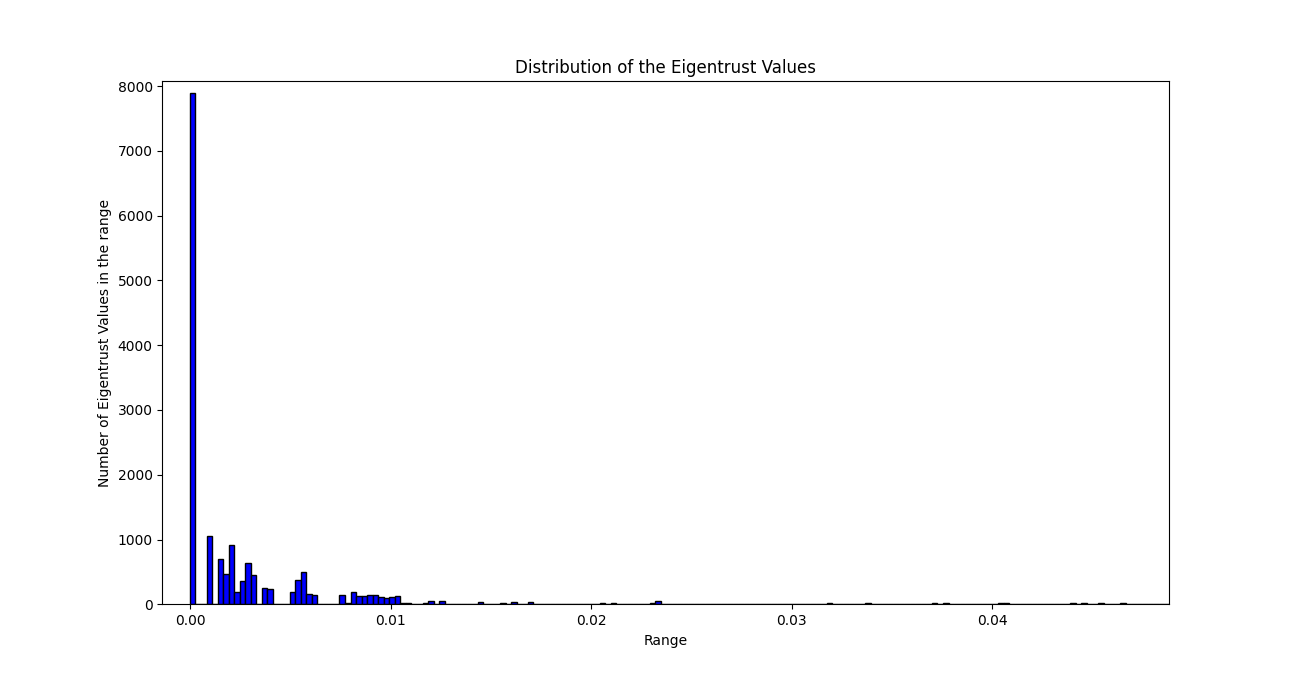
\includegraphics[scale=0.42]{eigentrust_distribution_detailed}
		\caption{Distribution of the Eigentrust Values before filtering. As can be seen nearly 17500 of the customers have zero eigentrust value.}
		\label{fig:eigentrust_distribution_figure}
	\end{figure}

	\subsubsection{Filterer Module} The Filterer Module is responsible for;
	\begin{itemize}
		\item Getting transaction/Eigentrust records for each community from the Neo4j database via Neo4j driver
		\item Calculating cosine similarities between customers in the same community
		\item Calculating weights between customers in the same community
		\item If the dataset consists of implicit ratings calculating recommendation coefficients otherwise making predictions for products
		\item Selecting k-products with the highest coefficients/predictions to recommend for each customer
	\end{itemize}

	\paragraph{Calculating Weights} \mbox{}\\
	\begin{equation*} 
	\begin{split}
	w_{c_{target}}(c_{2}) = \frac{2*sim(c_{target},c_{2})*trust(c_{2})}{sim(c_{target},c_{2})+trust(c_{2})}
	\end{split}
	\end{equation*}
	where $sim(c_{target},c_{2})$ represents "cosine similarity" between customers and $trust(c_{2})$ represents eigentrust belonged to $c_{2}$.

	\paragraph{Calculating Recommendation Coefficients}	
	\begin{equation*} 
	\begin{split}
	RC(i) = \frac{\sum_{c \in C}^{} w_{c_{target}}(c)*b_{c}}{\sum_{c \in C}^{} w_{c_{target}}(c)}
	\end{split}
	\end{equation*}
	where $RC(i)$ represents the recommendation coefficient calculated for product $i$ and $b_{c}$ is a boolean value which indicates whether the product was bought by person c or not.


	\paragraph{Making Predictions}
	\begin{equation*} 
	\begin{split}
	p(i) = \frac{\sum_{c \in C}^{} w_{c_{target}}(c)*r_{c}}{\sum_{c \in C}^{} w_{c_{target}}(c)}
	\end{split}
	\end{equation*}
	where $p(i)$ represents the prediction for product $i$ and $r_{c}$ represents rating given by customer $c$ for product $i$. $C$ customer set only contains the customers who purchased product i. \\
	
	
	\textbf{Important remark:} $C$ community set used in above functions consists only of customers belonged to the same community with $c_{target}$ while there is no such restriction in \ref{inverse_section}.

	\subsubsection{Recommender Module} Recommender Module is responsible for writing. The module has two tasks:
	\begin{enumerate}
		\item Getting the recommendation list that contains ids of the customers and corresponding recommended products from the Filterer module and writing these recommendations to the Neo4j database as a relationship between the customer and the recommended product using Neo4j driver.
	\end{enumerate}